% Slides for 2024-08-06
% To create a slide, use the following:
\begin{frame}{Approach :(}
    \begin{itemize}
        \item colab 
              A100, L4, T4, TPU
        \item nautilus 
              Kubernetes 
              NVIDIA-GeForce-RTX-2080-Ti, NVIDIA-L40, NVIDIA-GeForce-RTX-3090
    \end{itemize}
\end{frame}

\begin{frame}{Refactor}
    \begin{itemize}
        \item
              adjust size
        \item
              remove the ray.tune
        \item
              fixed hyper-param: LR - (1e-4, 2e-4) 
    \end{itemize}
\end{frame}

\begin{frame}{Refactor}
    \begin{figure} 
        \centering
        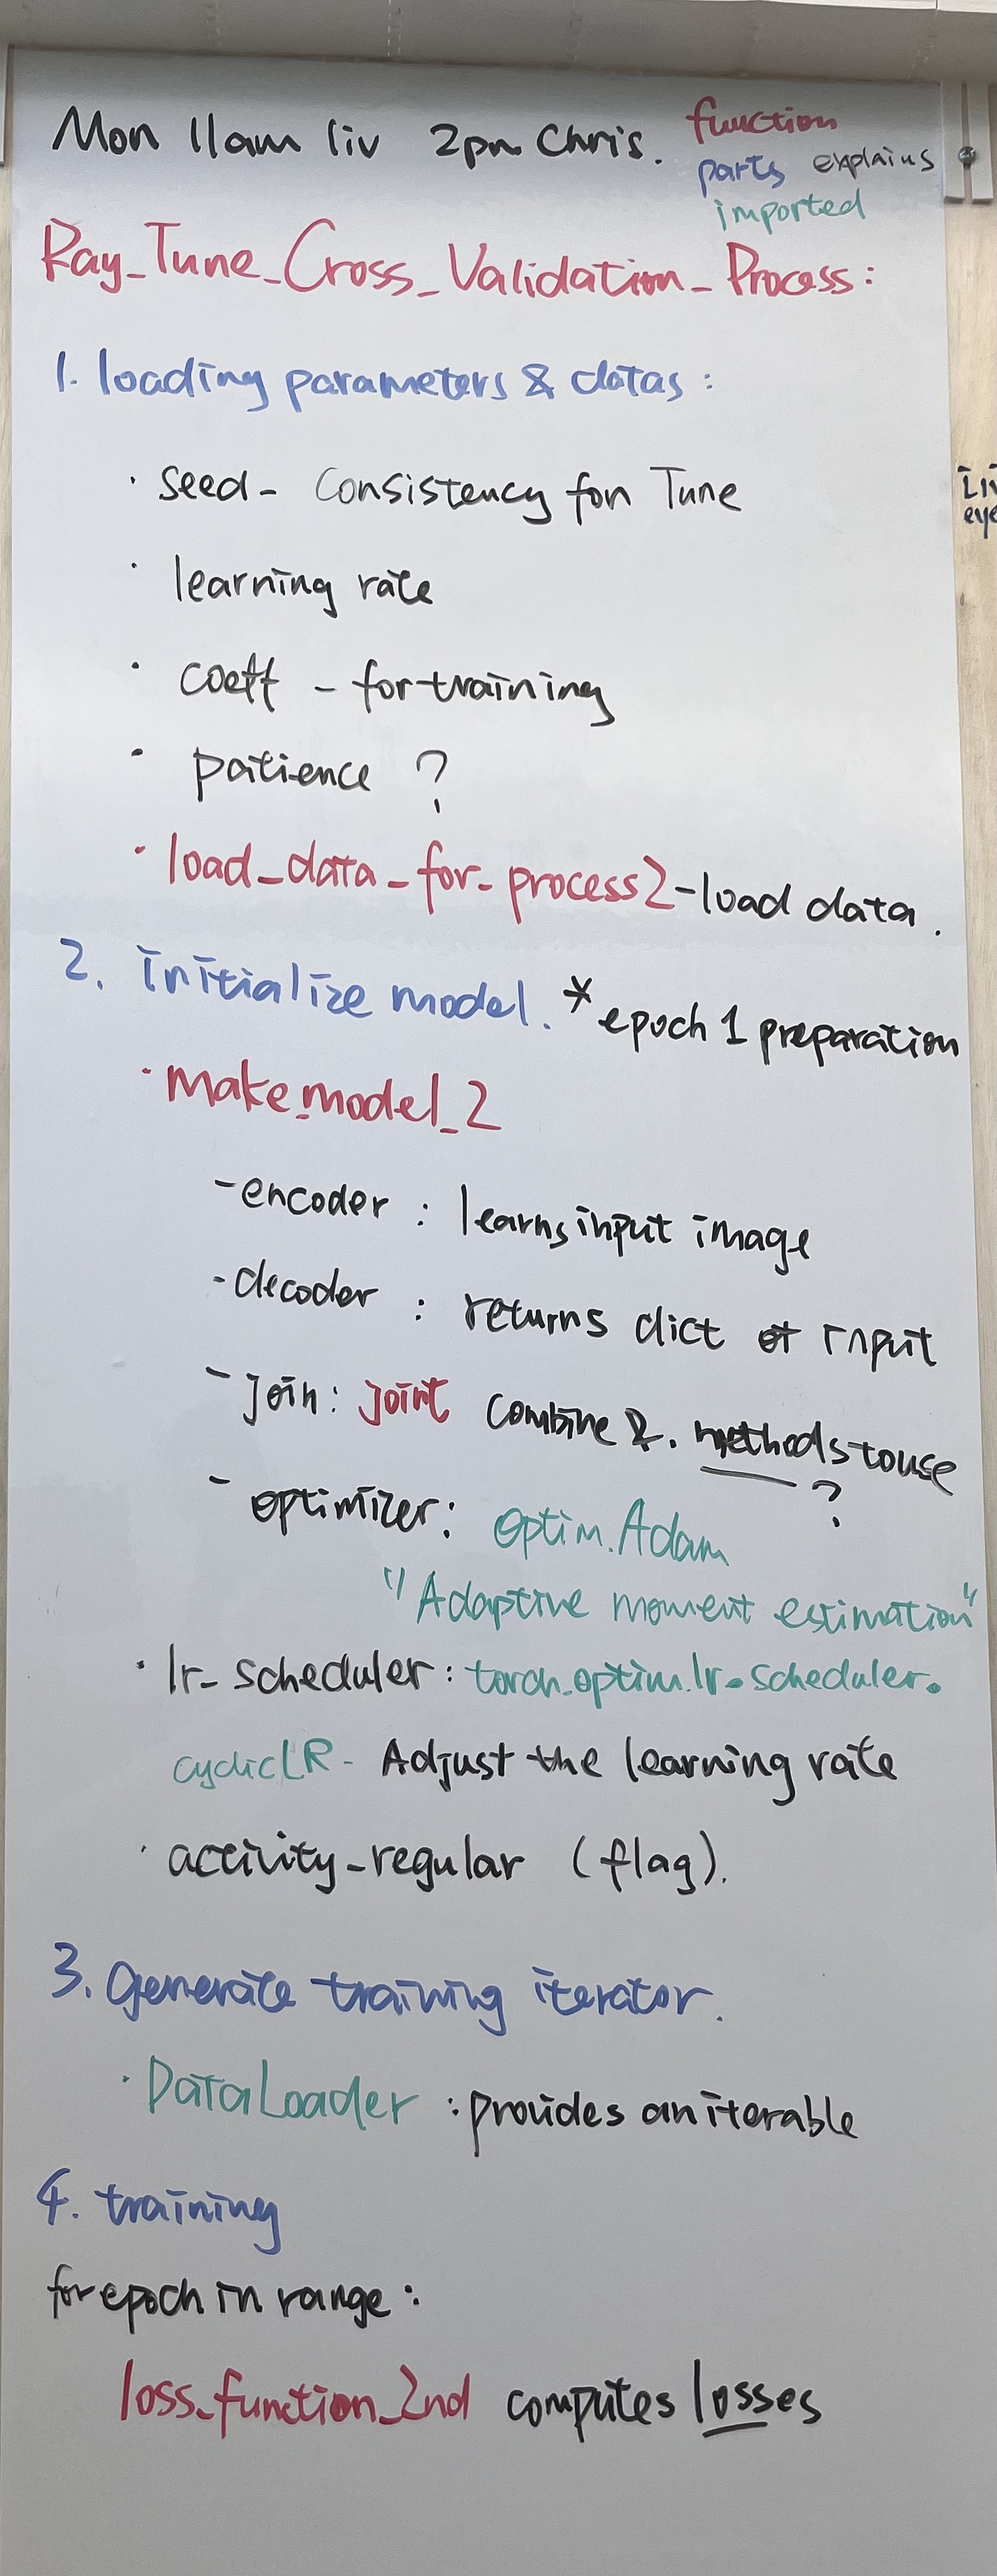
\includegraphics[width=0.2\linewidth]{images/IMG_4668.jpeg} 
    \end{figure}
\end{frame}

\begin{frame}{To-do}
    \begin{itemize}
        \item try 0\%, 25\%, 50\% noise for testing
        \item try 0\%, 25\%, 50\% noise for training and testing
    \end{itemize}
\end{frame}
% To create a slide with a bullet list, use the following:
% \begin{frame}{TITLE}
%     \begin{itemize}
%         \item ITEM 1
%         \item ITEM 2
%     \end{itemize}    
% \end{frame}

% To create a slide with numbered list, use the following:
% \begin{frame}{TITLE}
%     \begin{enumerate}
%         \item ITEM 1
%         \item ITEM 2
%     \end{enumerate}
% \end{frame}

% To create a slide with a graphic:
% 1. Add the graphic to this folder (named picture.png)
% 2. Use the following:
% \begin{frame}{TITLE}
%     \centering
%     \includegraphics[height=0.7\textheight,width=0.7\textwidth,keepaspectratio]{picture.png}
% \end{frame}

% To create a slide with two columns, use the following:
% \begin{frame}{TITLE}
%     \begin{columns}
%         \begin{column}{0.5\textwidth}
%             COLUMN 1 BODY
%         \end{column}
%         \begin{column}{0.5\textwidth}
%             COLUMN 2 BODY
%         \end{column}
%     \end{columns}
% \end{frame}
